\subsection{Mosaico} \label{sec:mosaico}

Transformação em mosaico da imagem por uma reordenação dos seus blocos. O argumento \texttt{ORDENACAO} deve conter uma caminho para o arquivo com essa nova ordenação e deve aparecer na sequência após o comando \texttt{mosaico}, como no invocação a seguir.

\begin{minted}{text}
    $ python main.py imagens/baboon.png mosaico padrao.txt
\end{minted}

\begin{figure}[H]
    \centering
    \begin{subfigure}{0.45\textwidth}
        \centering
        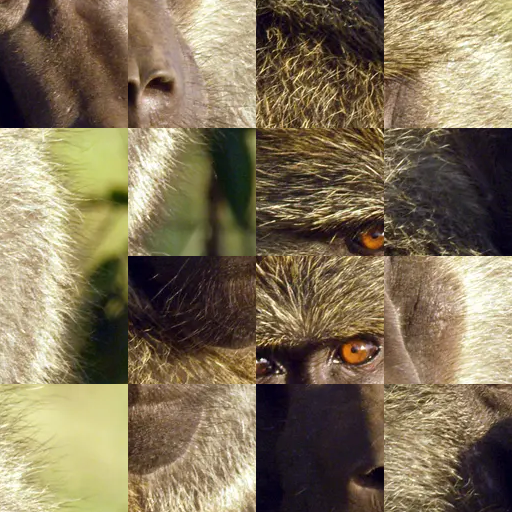
\includegraphics[width=6cm]{resultados/colormsc.png}
        \caption{\texttt{imagens/color.png}}
    \end{subfigure}%
    \begin{subfigure}{0.45\textwidth}
        \centering
        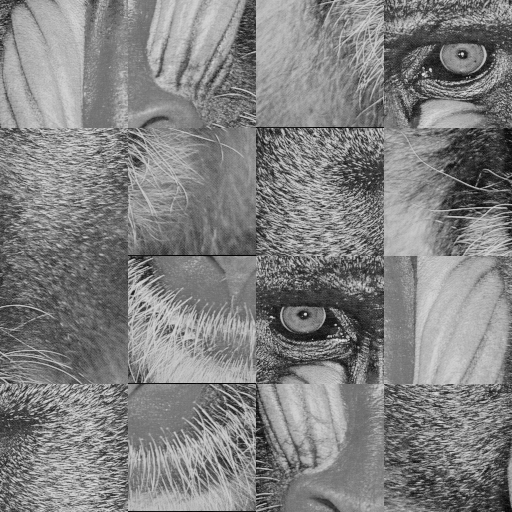
\includegraphics[width=6cm]{resultados/baboonmsc.png}
        \caption{\texttt{imagens/babooon.png}}
        \label{fig:res:10}
    \end{subfigure}

    \caption{Mosaico da imagem pelo \texttt{padrao.txt}.}
\end{figure}

\begin{listing}[H]
    \begin{minted}{python}
        def mosaico(imagem, ordem):
            N, M = ordem.shape
            # split e flatten
            bloco = [
                bloco
                for lin in np.vsplit(imagem, N)
                for bloco in np.hsplit(lin, M)
            ]
            # accesso (em lista) e concatena
            imagem = np.concatenate([
                np.concatenate([bloco[i-1] for i in lin], axis=1)
                for lin in ordem
            ])
            return imagem
    \end{minted}

    \caption{Comando \texttt{mosaico ORDENACAO}}
    \label{code:mosaico}
\end{listing}

O arquivo de reordenação deve ser composto de inteiros únicos entre $1$ e $N \times M$, dispostos em $N$ linhas e $M$ colunas, e separados apenas por espaços (para a leitura com \pyline{np.loadtxt} \autocite{ref:loadtxt}). As dimensões de tamanho da imagem também devem ser divisíveis por $N$ e $M$ (altura por $N$ e largura pro $M$) para que os blocos possam ser reposicionados. No código fonte existe um arquivo \texttt{padrao.txt} com a reordenação do enunciado para imagens com dimensões múltiplas de 4.

\begin{listing}[H]
    \begin{minted}{text}
        6 11 13  3
        8 16  1  9
       12 14  2  7
        4 15 10  5
    \end{minted}

    \caption{Arquivo \texttt{padrao.txt} com a reordenação proposta no enunciado.}
\end{listing}

Como a ordem do mosaico da imagem depende da entrada, o código não foi vetorizado, como pode ser visto no \hyperref[code:mosaico]{trecho \ref*{code:mosaico}}.
